\chapter{From the Burridge--Knopoff model to a sandpile}
\label{ch:mapping}

\newcommand{\mapSandDistEnd}{1.0e-12}
\newcommand{\mapLyapPlate}{47}
\newcommand{\mapperFixed}{25{,}376}
\newcommand{\mapperPlateFixed}{0.04248}
\newcommand{\mapperTopplingsFixed}{73.0}
\newcommand{\mapperReset}{152}
\newcommand{\mapperPlateReset}{0.07565}
\newcommand{\mapperTopplingsReset}{130.0}
\newcommand{\mapdropAthreeLsix}{0.04248}
\newcommand{\mapnoiseMaxfixedsix}{125}
\newcommand{\mapnoiseMeanfixedsix}{8.7}
\newcommand{\mapnoiseMaxMfixedsix}{0.24}
\newcommand{\mapnoiseMaxresetsix}{132}
\newcommand{\mapnoiseMeanresetsix}{8.3}
\newcommand{\mapnoiseMaxMresetsix}{0.40}
\newcommand{\mapnoiseMaxfixedtwelve}{247}
\newcommand{\mapnoiseMeanfixedtwelve}{15.0}
\newcommand{\mapnoiseMaxMfixedtwelve}{0.12}
\newcommand{\mapnoiseMaxresettwelve}{267}
\newcommand{\mapnoiseMeanresettwelve}{14.3}
\newcommand{\mapnoiseMaxMresettwelve}{0.20}
\newcommand{\mapbkaBlBAevents}{8{,}600{,}000}
\newcommand{\mapbkaBlBAmaxblocks}{2971}
\newcommand{\mapbkaBlBAplate}{501}
\newcommand{\mapbkaBlBEevents}{7{,}800{,}000}
\newcommand{\mapbkaBlBEmaxblocks}{6769}
\newcommand{\mapbkaBlBEplate}{511}
\newcommand{\mapbkaBlGevents}{5{,}600{,}000}
\newcommand{\mapbkaBlGmaxblocks}{1500}
\newcommand{\mapbkaBlGplate}{517}
\newcommand{\mapbkaDlBCevents}{5{,}000{,}000}
\newcommand{\mapbkaDlBCmaxblocks}{7359}
\newcommand{\mapbkaDlBCplate}{1018}
\newcommand{\mapbkaDlGevents}{3{,}000{,}000}
\newcommand{\mapbkaDlGmaxblocks}{2550}
\newcommand{\mapbkaDlGplate}{1048}
\newcommand{\mapbkaDlIevents}{3{,}000{,}000}
\newcommand{\mapbkaDlImaxblocks}{3178}
\newcommand{\mapbkaDlIplate}{1033}
\newcommand{\mapfixedaBlBAevents}{1{,}099{,}800{,}000}
\newcommand{\mapfixedaBlBAmaxblocks}{121}
\newcommand{\mapfixedaBlBAplate}{300}
\newcommand{\mapfixedaBlGevents}{305{,}200{,}000}
\newcommand{\mapfixedaBlGmaxblocks}{42}
\newcommand{\mapfixedaBlGplate}{300}
\newcommand{\mapfixedaDlBCevents}{1{,}078{,}200{,}000}
\newcommand{\mapfixedaDlBCmaxblocks}{87}
\newcommand{\mapfixedaDlBCplate}{300}
\newcommand{\mapfixedaDlGevents}{172{,}600{,}000}
\newcommand{\mapfixedaDlGmaxblocks}{69}
\newcommand{\mapfixedaDlGplate}{300}
\newcommand{\mapfixedaDlIevents}{276{,}200{,}000}
\newcommand{\mapfixedaDlImaxblocks}{65}
\newcommand{\mapfixedaDlIplate}{300}
\newcommand{\mapnoisefixedwApABlBCevents}{292{,}000{,}000}
\newcommand{\mapnoisefixedwApABlBCmaxblocks}{266}
\newcommand{\mapnoisefixedwApABlBCplate}{300}
\newcommand{\mapnoisefixedwApABlGevents}{89{,}400{,}000}
\newcommand{\mapnoisefixedwApABlGmaxblocks}{138}
\newcommand{\mapnoisefixedwApABlGplate}{300}
\newcommand{\mapnoisefixedwApAFlBCevents}{166{,}000{,}000}
\newcommand{\mapnoisefixedwApAFlBCmaxblocks}{265}
\newcommand{\mapnoisefixedwApAFlBCplate}{300}
\newcommand{\mapnoisefixedwApAFlGevents}{60{,}000{,}000}
\newcommand{\mapnoisefixedwApAFlGmaxblocks}{130}
\newcommand{\mapnoisefixedwApAFlGplate}{301}
\newcommand{\mapnoisefixedwApClBCevents}{80{,}400{,}000}
\newcommand{\mapnoisefixedwApClBCmaxblocks}{247}
\newcommand{\mapnoisefixedwApClBCplate}{300}
\newcommand{\mapnoisefixedwApClGevents}{30{,}000{,}000}
\newcommand{\mapnoisefixedwApClGmaxblocks}{125}
\newcommand{\mapnoisefixedwApClGplate}{301}
\newcommand{\mapnoiseresetwApABlBCevents}{117{,}800{,}000}
\newcommand{\mapnoiseresetwApABlBCmaxblocks}{413}
\newcommand{\mapnoiseresetwApABlBCplate}{300}
\newcommand{\mapnoiseresetwApABlGevents}{50{,}200{,}000}
\newcommand{\mapnoiseresetwApABlGmaxblocks}{991}
\newcommand{\mapnoiseresetwApABlGplate}{301}
\newcommand{\mapnoiseresetwApAFlBCevents}{138{,}400{,}000}
\newcommand{\mapnoiseresetwApAFlBCmaxblocks}{276}
\newcommand{\mapnoiseresetwApAFlBCplate}{300}
\newcommand{\mapnoiseresetwApAFlGevents}{49{,}000{,}000}
\newcommand{\mapnoiseresetwApAFlGmaxblocks}{137}
\newcommand{\mapnoiseresetwApAFlGplate}{300}
\newcommand{\mapnoiseresetwApClBCevents}{51{,}000{,}000}
\newcommand{\mapnoiseresetwApClBCmaxblocks}{267}
\newcommand{\mapnoiseresetwApClBCplate}{301}
\newcommand{\mapnoiseresetwApClGevents}{22{,}000{,}000}
\newcommand{\mapnoiseresetwApClGmaxblocks}{132}
\newcommand{\mapnoiseresetwApClGplate}{302}
\newcommand{\mapresetaDlBCevents}{3{,}800{,}000}
\newcommand{\mapresetaDlBCmaxblocks}{8191}
\newcommand{\mapresetaDlBCplate}{311}
\newcommand{\mapresetaDlGevents}{600{,}000}
\newcommand{\mapresetaDlGmaxblocks}{4095}
\newcommand{\mapresetaDlGplate}{334}
\newcommand{\mapresetaDlIevents}{1{,}400{,}000}
\newcommand{\mapresetaDlImaxblocks}{4095}
\newcommand{\mapresetaDlIplate}{308}
\newcommand{\maptauAthreeLG}{1.962}
\newcommand{\maperrAthreeLG}{0.006}
\newcommand{\mapbAthreeLG}{0.96}
\newcommand{\maptauAthreeLI}{1.921}
\newcommand{\maperrAthreeLI}{0.004}
\newcommand{\mapbAthreeLI}{0.92}
\newcommand{\maptauAthreeLM}{1.913}
\newcommand{\maperrAthreeLM}{0.002}
\newcommand{\mapbAthreeLM}{0.91}
\newcommand{\maptauAoneLG}{1.400}
\newcommand{\maperrAoneLG}{0.001}
\newcommand{\mapbAoneLG}{0.40}
\newcommand{\maptauAoneLK}{1.363}
\newcommand{\maperrAoneLK}{0.001}
\newcommand{\mapbAoneLK}{0.36}
\newcommand{\maptauAoneLO}{1.357}
\newcommand{\maperrAoneLO}{0.001}
\newcommand{\mapbAoneLO}{0.36}


Chapter~\ref{ch:bk} ended with a list of ingredients that determine the statistics of the Burridge--Knopoff
(BK) model: a threshold with a drop of the force, redistribution of the shed force with partial loss into the
pulling springs, uniform driving, and inertia with velocity weakening. The first three are exactly the
ingredients of a sandpile model. In this chapter we make the correspondence precise: we derive a sandpile model
from the BK equations by removing inertia (\cref{sec:map-derivation}), study its properties
(\cref{sec:map-properties}), and then compare its statistics with those of the full BK model, simulated with the
same parameters (\cref{sec:map-comparison}). The comparison answers the central question of this thesis: which
features of the BK model survive the mapping, and which do not.

% ======================================================================
\section{Derivation}
\label{sec:map-derivation}

\subsection{The force variables}

The natural variable for a sandpile description is not the displacement $U_j$ of a block but the total spring force
acting on it,
\begin{equation}
  f_j = \ell^2\,(U_{j+1}-2U_j+U_{j-1}) + (P - U_j),
  \label{eq:fj}
\end{equation}
with free ends ($U_0\equiv U_1$, $U_{N+1}\equiv U_N$) and $P$ the position of the plate. A stuck block stays stuck as long as
$f_j<1$, and starts to slip when $f_j$ reaches 1: $f_j$ plays the role of the height of a sandpile site, and 1 is the critical
height.

Two properties of $f_j$ follow directly from \cref{eq:fj}.
\begin{enumerate}
  \item \textbf{Response to a slip.} If block $j$ moves forward by $\Delta$ while all other blocks stay where they are, its own
    force changes by $-(2\ell^2+1)\Delta$ (two coupling springs and its pulling spring resist the motion) and the force on each
    neighbour increases by $\ell^2\Delta$ (the coupling spring between them is compressed). For an end block, which has only one
    neighbour, the own force changes by $-(\ell^2+1)\Delta$. We write
    \begin{equation}
      \omega_j^2 = \begin{cases} 2\ell^2+1 & \text{bulk},\\ \ell^2+1 & \text{ends.}\end{cases}
    \end{equation}
  \item \textbf{Total force.} Summing \cref{eq:fj} over all blocks, the coupling terms cancel in pairs (each spring pushes one
    block as much as it pulls the other), so
    \begin{equation}
      \sum_{j=1}^N f_j = N P - \sum_{j=1}^{N} U_j .
      \label{eq:total-force}
    \end{equation}
    This identity is exact, in the full BK model as well. Since the moment of an event is $M = \sum_j\delta U_j$ (with $a=1$), it
    gives the force bookkeeping
    \begin{equation}
      \Delta\Bigl(\sum_j f_j\Bigr) = N\,\Delta P - \sum_{\text{events}} M .
      \label{eq:force-bookkeeping}
    \end{equation}
    The plate adds force $N\,\Delta P$; slip removes exactly as much force as its moment. Because the forces stay bounded, over a long
    time the total moment per block equals the plate displacement: this is the sum rule \cref{eq:sumrule}.
\end{enumerate}

\subsection{The quasi-static approximation}

The BK dynamics is replaced by a sequence of elementary slips under the following assumptions:
\begin{enumerate}[label=(A\arabic*)]
  \item \textbf{One block at a time.} A block that reaches the threshold slips while its neighbours are stuck, as in the one-block
    event of \cref{sec:one-block-event}.
  \item \textbf{A fixed slip.} Each such slip has the size of the one-block event, $\Delta_j = \Delta f/\omega_j^2$, where
    \begin{equation}
      \Delta f = \sigma\left(1+e^{\pi\alpha/\omega}\right),\qquad \omega = \sqrt{2\ell^2+1-\alpha^2},
      \label{eq:map-drop}
    \end{equation}
    is the force shed in a one-block event (\cref{eq:dU1-alpha}).
  \item \textbf{No memory of motion.} After its slip the block is at rest; its neighbours feel only the static change of force
    $\ell^2\Delta_j$. No kinetic energy or momentum is passed on.
  \item \textbf{Slow, uniform driving.} The plate moves only when all blocks are stuck, until the most loaded block reaches the threshold
    (the limit $\nu\to0$).
\end{enumerate}
Under these assumptions the BK model becomes a continuous sandpile on the chain:
\begin{description}[font=\normalfont\itshape]
  \item[Drive.] Raise all $f_j$ by the same amount until $\max_j f_j = 1$.
  \item[Toppling.] A site with $f_j\ge1$ topples: $f_j\to f_j - \Delta f$ and $f_{j\pm1}\to f_{j\pm1} + \ell^2\Delta f/\omega_j^2$. The
    corresponding block has slipped by $\Delta f/\omega_j^2$.
  \item[Avalanche.] Topplings continue until all $f_j<1$. Its moment is the sum of the slips.
\end{description}
\Cref{fig:toppling-map} illustrates the correspondence.

\begin{figure}[t]
\centering
\begin{tikzpicture}[x=10mm,y=10mm,>={Stealth[length=1.8mm]}]
  % plate
  \fill[cblue!12] (-0.3,2.3) rectangle (6.3,2.6); \draw[ink2] (-0.3,2.3) rectangle (6.3,2.6);
  \fill[pattern=north east lines,pattern color=ink2!50] (-0.3,-0.2) rectangle (6.3,0); \draw[ink2] (-0.3,0)--(6.3,0);
  \foreach \x/\c in {0.5/cblue!10,2.5/corange!25,4.5/cblue!10} {
    \draw[ink2,fill=\c] (\x,0) rectangle (\x+1,0.8);
    \draw[ink2,decorate,decoration={zigzag,segment length=2mm,amplitude=0.9mm}] (\x+0.5,0.8)--(\x+0.5,2.3);
  }
  \draw[ink2,decorate,decoration={zigzag,segment length=2mm,amplitude=0.9mm}] (1.5,0.4)--(2.5,0.4);
  \draw[ink2,decorate,decoration={zigzag,segment length=2mm,amplitude=0.9mm}] (3.5,0.4)--(4.5,0.4);
  \draw[->,corange,thick] (3.1,1.0)--(3.9,1.0) node[midway,above,font=\footnotesize] {slip $\Delta$};
  \node[font=\footnotesize,align=center] at (1.0,-0.6) {$+\ell^2\Delta$};
  \node[font=\footnotesize,align=center] at (3.0,-0.6) {$-(2\ell^2{+}1)\Delta$};
  \node[font=\footnotesize,align=center] at (5.0,-0.6) {$+\ell^2\Delta$};
  \node[font=\footnotesize,ink2,anchor=west] at (6.4,-0.6) {change of force $f$};
  \node[font=\footnotesize,ink2,anchor=west] at (6.4,1.6) {pulling spring takes $\Delta$};
  \draw[->,ink2] (6.35,1.6) -- (3.65,1.6);
  \node[font=\footnotesize,ink2,anchor=west] at (6.4,2.45) {plate};
\end{tikzpicture}
\caption{A slip $\Delta$ of one block while its neighbours are stuck, as a sandpile toppling. The block's own force drops by $(2\ell^2+1)\Delta$; each neighbour gains
$\ell^2\Delta$; the remaining $\Delta$ is taken up by the block's pulling spring and is lost to the chain. With $\Delta=\Delta f/(2\ell^2+1)$ the lost fraction of the shed
force is $\epsilon = 1/(2\ell^2+1)$.}
\label{fig:toppling-map}
\end{figure}

Of the force $\Delta f$ shed by a toppling in the bulk, a fraction $2\ell^2/(2\ell^2+1)$ goes to the neighbours, and the fraction
\begin{equation}
  \epsilon = \frac{1}{2\ell^2+1}
\end{equation}
is lost into the pulling spring. This model is the one used in the earlier version of this project (with $\Delta f$ expanded to first order in
$\alpha$, $\Delta f\approx\sigma(2+\pi\alpha/\omega)$); we call it the \emph{fixed-drop} rule.

\subsection{The Olami--Feder--Christensen variant}

Assumption (A2) can be replaced by another natural choice. A block whose force has been pushed \emph{above} the threshold by its neighbours
carries an excess force, and one may argue that it should slip until its force returns to a fixed residual value $f_r$:
\begin{equation}
  \Delta_j = \frac{f_j - f_r}{\omega_j^2},\qquad f_j\to f_r .
\end{equation}
This is the rule of Olami, Feder and Christensen (OFC)~\cite{OFC1992}, who derived it from a two-dimensional BK model by the same removal of
inertia; in their language the ``conservation level'' is $\ell^2/(2\ell^2+1)$ per neighbour. We call it the \emph{reset} rule and choose
$f_r = 1-\Delta f$, so that a toppling exactly at threshold sheds the same force as in the fixed-drop rule. The two rules differ only for
sites that are pushed above the threshold during an avalanche.

% ======================================================================
\section{Properties of the mapped model}
\label{sec:map-properties}

\paragraph{The fixed-drop rule is Abelian.} Every toppling of site $j$ changes the forces by the same fixed vector (minus $\Delta f$ at $j$, plus
$\ell^2\Delta f/\omega_j^2$ at each neighbour). This is exactly the structure of the BTW model, with real numbers instead of integers, and the
proof of \cref{thm:abelian} applies word for word: the final configuration and the number of topplings of every site do not depend on the order of
topplings. The reset rule is not Abelian, because the size of a toppling depends on the force at the moment it happens; for it we use the parallel
update of Chapter~\ref{ch:soc}.

\paragraph{The drop only sets the units.} Since the threshold is the same for all sites and the drive is uniform, only the differences $f_j - 1$
matter. Measuring them in units of $\Delta f$, i.e.\ setting $\hat f_j = (f_j-1)/\Delta f$, the toppling rule becomes $\hat f_j\to\hat f_j-1$,
$\hat f_{j\pm1}\to\hat f_{j\pm1}+\ell^2/\omega_j^2$, which no longer contains $\Delta f$. The sequence of avalanches, measured by the number of
topplings, therefore depends only on $\ell$ (and $N$). The friction parameters $\alpha$ and $\sigma$ enter only through $\Delta f$, i.e.\ through the
\emph{unit} in which slips are measured: every moment is proportional to $\Delta f$, and changing $\alpha$ or $\sigma$ shifts the whole distribution
of $\mu = \ln M$ by $\ln\Delta f$ without changing its shape.

This is a sharp prediction, and it is opposite to the behaviour of the BK model. In the BK model $\alpha$ controls the localization length
$\tilde\xi\propto(\xi/\alpha)\ln(4\ell^2/\sigma)$ and the shape of the distribution: Carlson \emph{et al.} found $b\approx1$ with a separate peak of
delocalized events for $\alpha=3$, but a single power law with $b\approx0.35$ for $\alpha=1$. If the mapping were complete, both would collapse onto
one curve after a shift in $\mu$.

\paragraph{The sum rule.} The force bookkeeping \cref{eq:force-bookkeeping} holds exactly in the mapped model as well: a toppling of site $j$ removes
$\omega_j^2\Delta_j$ from $f_j$ and adds $\ell^2\Delta_j$ to each neighbour, a net change of $-\Delta_j$ in both the bulk and at the ends. Hence the
total moment per block again equals the plate displacement, and the frequencies $\mathcal D(\mu)$ of the two models are normalised in the same way
and can be compared directly.

\paragraph{Number of topplings per unit plate displacement.} Per unit displacement of the plate, each block must slip by one unit on average. With the
fixed-drop rule every bulk toppling is a slip of $\Delta f/(2\ell^2+1)$, so each site topples on average $(2\ell^2+1)/\Delta f$ times per unit plate
displacement. For $\ell=6$, $\alpha=3$, $\sigma=0.01$ ($\Delta f\approx0.042$) this is about 1700 topplings per site, compared with a single slip of
order one in a great event of the BK model. The mapped model must accomplish with many small steps what the BK model does with few large ones.

\section{Simulations: the BK model against its sandpile limit}
\label{sec:map-comparison}

\subsection{Set-up}

All simulations use the programs described in Chapter~6. The BK model is simulated in the limit $\nu\to0$ with the 1991 friction law. We use
the parameters of Carlson \emph{et al.}~\cite{Carlson1991}: $\alpha=3$, $\sigma=0.01$, $\ell = 6$, 8 and 12 (their Fig.~3), and $\alpha=1$,
$\sigma=0.01$, $\ell=6$, 10 and 14 (their Fig.~6), with $N=4096$ blocks for $\ell<10$ and $N=8192$ otherwise. Each run starts from a
slightly irregular configuration, discards a transient of 200 units of plate displacement, and then records every event during the next 1000
units (500 for $\alpha=1$), i.e.\ $3\times10^6$ to $9\times10^6$ events. The sandpile models are run with the same $N$ and $\ell$ and with
$\Delta f$ given by \cref{eq:map-drop}; they need about $10^6$ avalanches per unit of plate displacement, and we record 300 units after a
transient of 100. In every run the sum rule \cref{eq:sumrule} is satisfied to better than $3\times10^{-4}$. As in the papers, distributions are
shown as $\ln[\xi\,\mathcal D(\mu)]$ against $\ln(M/\xi)$, with $\xi=\ell$ (block spacing $a=1$).

\subsection{The BK model reproduces the published results}

\Cref{fig:compare} (blue curves) shows the distributions of the BK model. They have all the features described by Carlson \emph{et al.}: peaks
of one- and few-block events at the left, a straight scaling region of localized events, a minimum just below $M=\xi$, a rising branch of
delocalized events, and a sharp upper cutoff; the largest events involve about half of the chain or less. To measure the exponents we follow the
procedure of \cref{sec:protocol}. \Cref{fig:bk-effective} shows the effective exponent $\tau_{\text{eff}}$ of the moment density $P(M)$, obtained by
maximum-likelihood fits in sliding one-decade windows.
\begin{itemize}
  \item For $\alpha=3$, $\tau_{\text{eff}}$ is flat over two decades, $10^{-4}\xi<M<10^{-2}\xi$, for all three values of $\ell$. Fits in this window
    give $\tau = \maptauAthreeLG\pm\maperrAthreeLG$, $\maptauAthreeLI\pm\maperrAthreeLI$ and $\maptauAthreeLM\pm\maperrAthreeLM$ for $\ell=6$, 8
    and 12, i.e.\ $b=\tau-1 = \mapbAthreeLG$, $\mapbAthreeLI$, $\mapbAthreeLM$, in agreement with the value $b\approx0.92$ quoted by Carlson
    \emph{et al.} (from a least-squares fit). Above $M\approx10^{-2}\xi$ the exponent decreases and reaches $\tau_{\text{eff}}\approx0$ at
    $M\approx5\xi$: there $P(M)$ is flat, which is the rising branch $\mathcal D\propto M$ ($b'=-1$) of \cref{eq:D91}.
  \item For $\alpha=1$, $\tau_{\text{eff}}$ is nearly constant over five decades. Fits in $10^{-3}\xi<M<\xi$ give $\tau = \maptauAoneLG$,
    $\maptauAoneLK$ and $\maptauAoneLO$ for $\ell=6$, 10 and 14, i.e.\ $b\approx\mapbAoneLG$--$\mapbAoneLO$, close to the single power law with
    $b\approx0.35$ found by Carlson \emph{et al.}
\end{itemize}
Our implementation therefore reproduces the 1991 results quantitatively, which is the precondition for using it as a reference. (Chapter~7
returns to the reproduction in more detail, including the 1989 model.)

\begin{figure}[t]
  \centering
  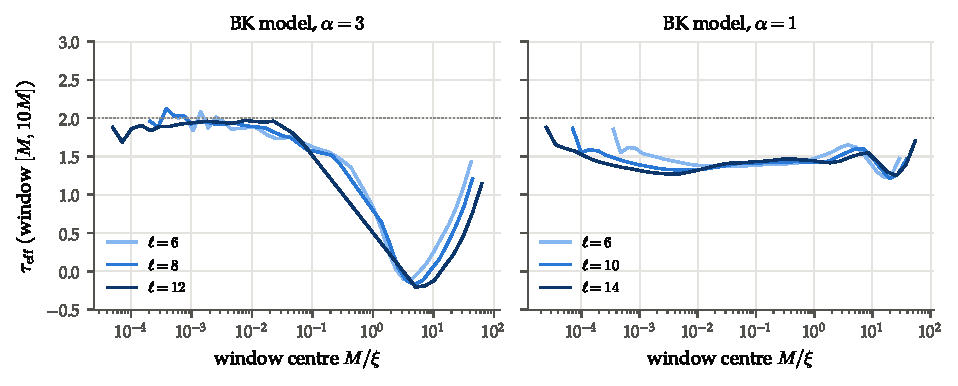
\includegraphics[width=\linewidth]{mapping/bk_effective.pdf}
  \caption{Effective exponent of the moment density of the BK model, from maximum-likelihood fits in windows $[M,10M]$. The dotted line marks
  $\tau=2$, i.e.\ $b=1$.}
  \label{fig:bk-effective}
\end{figure}

\subsection{The sandpile limit is periodic}

The sandpile models behave in a completely different way. Their dynamics, after a transient, is \emph{exactly periodic}: the same sequence of
avalanches repeats again and again. For $N=4096$ and $\ell=6$, the fixed-drop rule has a period of $\mapperFixed$ avalanches, during which the plate
advances by exactly $\mapperPlateFixed$, which is the drop $\Delta f = \mapdropAthreeLsix$, and every site topples on average $\mapperTopplingsFixed$ times.
The reason is simple. Every toppling changes the forces by a fixed amount, $-\Delta f$ at the toppling site and $+\ell^2\Delta f/\omega_j^2$ at its
neighbours, and the plate adds a uniform amount. Up to an overall shift, the forces therefore live on a discrete grid; since they are also bounded,
the deterministic dynamics can visit only a finite number of configurations and must eventually repeat itself. The number of topplings per period
follows from force balance: in one period each bulk site gains $\Delta f$ from the plate, so it must topple $n$ times with
$n\Delta f(1 - 2\ell^2/\omega^2) = \Delta f$, i.e.\ $n = 2\ell^2+1 = 73$ for $\ell = 6$.

The reset (OFC) rule is periodic as well (period $\mapperReset$ avalanches for the same parameters), but in a different way: it
\emph{synchronises}. Almost every avalanche topples nearly all sites of the chain once; the system fires as a whole, like the single block of
\cref{fig:single-block}. This synchronisation of OFC-type models under uniform deterministic driving is well known.

The BK model, by contrast, is chaotic. \Cref{fig:chaos} follows two copies of each model that start from configurations differing by $10^{-12}$ in the
position of a single block. In the BK model the difference stays at $10^{-12}$ until an event reaches the perturbed block, and then grows by ten orders
of magnitude within about one unit of plate displacement. In the sandpile the difference is simply carried along, without growing, for as long as we
follow it. This is the dynamical difference between the two models: the velocity-weakening instability of \cref{sec:bk-instability} continuously
generates new irregularities in the BK chain, while the inertia-free sandpile has no such source and settles on a periodic orbit.

\begin{figure}[t]
  \centering
  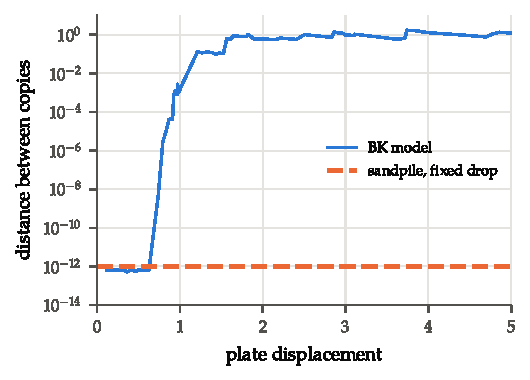
\includegraphics[width=0.55\linewidth]{mapping/chaos.pdf}
  \caption{Sensitivity to initial conditions. Distance between two copies of each model that initially differ by $10^{-12}$ in one block ($N=256$,
  $\ell=6$, $\alpha=3$, $\sigma=0.01$).}
  \label{fig:chaos}
\end{figure}

\subsection{Distributions}

\Cref{fig:compare} compares the distributions of the three models. The fixed-drop sandpile produces only small avalanches: their moments lie between that of a
one-block event and about $10^{-2}\xi$, and they involve at most a few tens of blocks (\cref{fig:blocks}), comparable to the stiffness length $\ell$. There is no
scaling region, no crossover and no delocalized events: the distribution is a single hump. The reset sandpile shows a few sharp spikes, the sizes that occur in its
synchronised cycle; the largest correspond to the whole chain slipping. Neither resembles the BK distribution, which extends continuously over more than seven
decades in moment.

\begin{figure}[t]
  \centering
  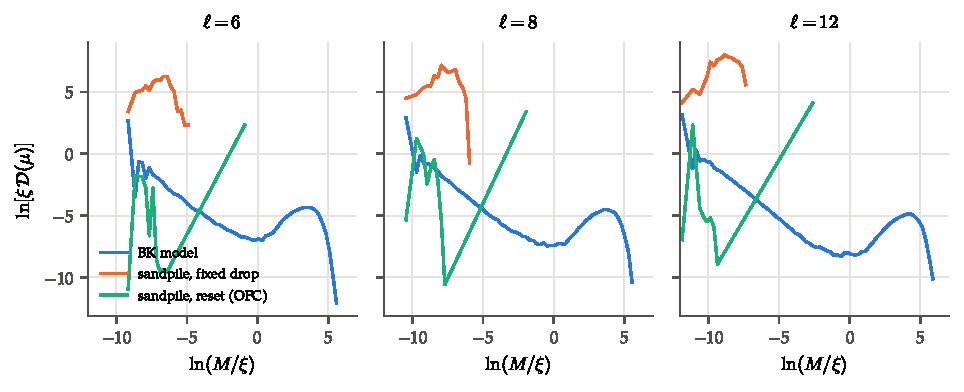
\includegraphics[width=\linewidth]{mapping/compare_alpha3.pdf}
  \caption{Frequency of events per unit magnitude, per unit length and per unit plate displacement, for the BK model and its two sandpile limits ($\alpha=3$,
  $\sigma=0.01$). The curves of the reset rule consist of a few spikes, the distinct sizes in its periodic, synchronised cycle.}
  \label{fig:compare}
\end{figure}

\begin{figure}[t]
  \centering
  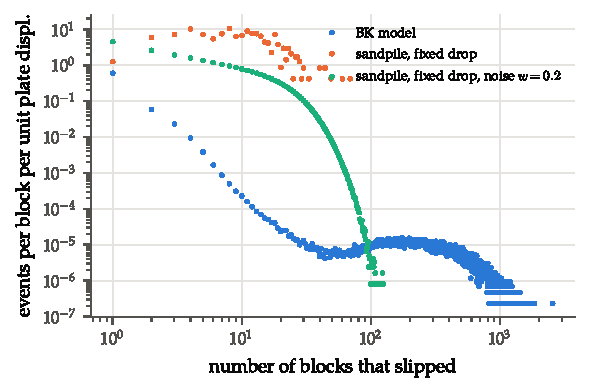
\includegraphics[width=0.62\linewidth]{mapping/blocks.pdf}
  \caption{Distribution of the number of blocks that slip in an event, for $\ell=6$, $\alpha=3$, $\sigma=0.01$.}
  \label{fig:blocks}
\end{figure}

\subsection{The test with \texorpdfstring{$\alpha$}{alpha}}

\Cref{sec:map-properties} predicted that in the sandpile limit the friction parameters only set the unit of slip. \Cref{fig:alpha-test} confirms this: for $\ell=6$, the
sandpile distributions for $\alpha=1$ and $\alpha=3$ nearly coincide once $\mu$ is measured relative to $\ln\Delta f$ (the remaining small differences come from the two
runs having settled on different periodic orbits). In the BK model the same change of $\alpha$ transforms the distribution: for $\alpha=3$ it has a steep scaling region and
a separate peak of large events, for $\alpha=1$ a single, much flatter power law. The dependence on $\alpha$, i.e.\ on how strongly a slipping block accelerates, is a
property of the inertial dynamics that the sandpile limit cannot represent.

\begin{figure}[t]
  \centering
  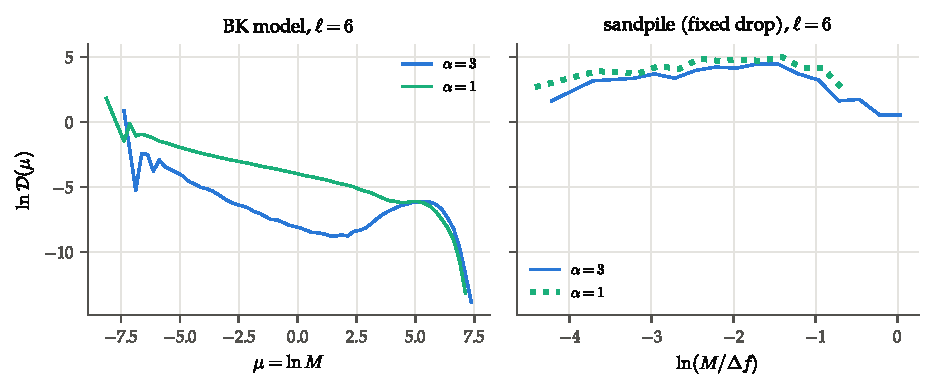
\includegraphics[width=\linewidth]{mapping/alpha_test.pdf}
  \caption{Changing the velocity weakening $\alpha$ at $\ell=6$, $\sigma=0.01$. Left: BK model. Right: fixed-drop sandpile, with moments measured in units of the drop
  $\Delta f$.}
  \label{fig:alpha-test}
\end{figure}

\subsection{Adding disorder}

The periodicity of the sandpile limit suggests a possible repair. In the BK model, irregularities are generated by the dynamics itself; in the sandpile
they could be supplied from outside. A common way to do this is to give the friction a random component: each block has its own static threshold
$\theta_j$, and after every slip it draws a new one, $\theta_j = 1+\eta$ with $\eta$ uniformly distributed in $[-w/2,w/2]$. This models a fault surface
whose strength varies from place to place and changes as the surface slides. We used $w = 0.01$, $0.05$ and $0.2$, i.e.\ from a quarter of the drop
$\Delta f$ to about five times it.

The noise destroys the periodicity of both rules, and for $w\ge0.05$ it also destroys the synchronisation of the reset rule. The distributions become smooth
(\cref{fig:noise}), but they remain bounded: even for the strongest noise the largest events involve $\mapnoiseMaxfixedsix$ blocks for $\ell=6$ and
$\mapnoiseMaxfixedtwelve$ for $\ell=12$ (fixed-drop rule), with moments below about $\mapnoiseMaxMfixedsix\,\xi$, and the mean number of blocks per event is
$\mapnoiseMeanfixedsix$ and $\mapnoiseMeanfixedtwelve$. The size of the largest events thus grows in proportion to the stiffness length, as expected from the bulk
dissipation $\epsilon = 1/(2\ell^2+1)$ discussed in \cref{sec:soc-implications}: a packet of force that loses a fraction $\epsilon$ at each toppling
travels a distance of order $\epsilon^{-1/2}\approx\sqrt2\,\ell$. None of the noisy sandpiles develops a scaling region, a crossover or delocalized events.

\begin{figure}[t]
  \centering
  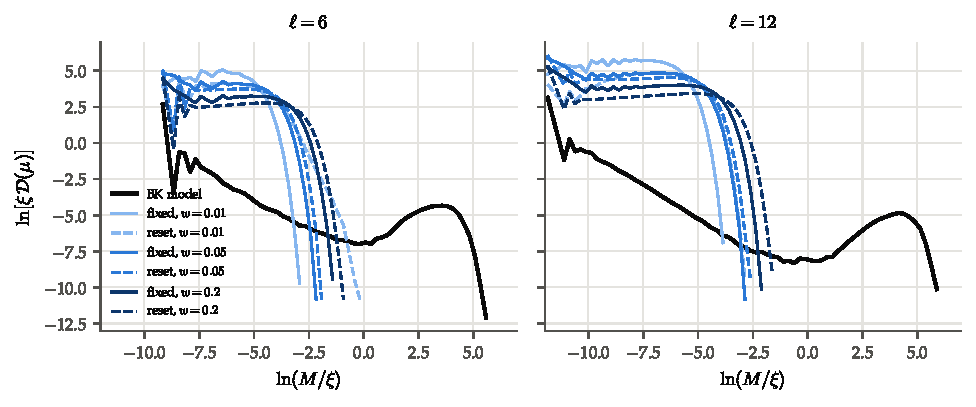
\includegraphics[width=\linewidth]{mapping/noise.pdf}
  \caption{The sandpile limit with random thresholds (noise width $w$), compared with the BK model ($\alpha=3$, $\sigma=0.01$). Solid: fixed-drop rule;
  dashed: reset rule.}
  \label{fig:noise}
\end{figure}

% ======================================================================
\section{What the mapping captures and what it misses}
\label{sec:map-discussion}

The comparison gives a clear answer to the question posed at the beginning of this chapter.

\paragraph{What survives.} The mapping is exact for the elementary process: an isolated toppling of the sandpile is, by construction, identical to a
one-block event of the BK model, including the velocity-weakening correction \cref{eq:map-drop}, and the smallest events of the two models agree to about 1\% (the remaining difference is the curvature of the friction law, which \cref{eq:map-drop} neglects). The
force bookkeeping \cref{eq:force-bookkeeping} and the sum rule are exact in both. The redistribution of the shed force, with the fraction
$\epsilon=1/(2\ell^2+1)$ lost into the pulling springs, is also the same.

\paragraph{What is lost.} Everything that depends on the \emph{motion} of the blocks is lost:
\begin{enumerate}
  \item \textbf{Amplification of slip.} In the BK model a slip that spreads gains energy, because velocity-weakening friction acts as a negative damping
    (\cref{sec:bk-pulses}). A group of blocks slips further than a single block, and a pulse that runs through a region near threshold grows exponentially.
    This is what produces the delocalized events and the localization length $\tilde\xi$. In the sandpile every toppling sheds the same small force,
    whatever its neighbours are doing, so avalanches cannot grow beyond the range set by the bulk dissipation, about $\ell$ blocks.
  \item \textbf{Self-generated disorder.} The same instability makes the BK model chaotic (\cref{fig:chaos}); the large events leave behind rough
    configurations whose smoothing produces the scaling region of localized events (\cref{sec:bk-events}). The inertia-free sandpile is not chaotic: it
    settles on a periodic orbit, and externally imposed disorder does not replace the missing amplification.
  \item \textbf{The dependence on $\alpha$.} Because the sandpile only knows the drop $\Delta f$, it cannot distinguish strong from weak velocity weakening,
    which in the BK model changes the exponent of the scaling region from $b\approx1$ to $b\approx0.4$.
\end{enumerate}

\paragraph{Conclusion.} The simple quasi-static mapping of the one-dimensional BK model onto a sandpile \emph{fails}: the sandpile limit is neither critical
nor chaotic, and it reproduces none of the features of the BK size distribution beyond the smallest events. The failure is not a matter of parameters or of
details of the toppling rule: both natural rules (fixed drop and OFC reset) fail, with and without noise. It is a consequence of removing inertia, which in
the BK model is the mechanism that makes events grow. A cellular-automaton description of the BK model would have to represent this amplification:
a slipping region gains momentum as it grows, and the blocks it reaches are pushed not only by the static forces of the springs but by moving
neighbours. Representing momentum requires carrying the velocities of the blocks from one step to the next, which brings back the full dynamics of
\cref{eq:bk}. In this sense the statistics of the BK model are intrinsically dynamical: they cannot be obtained from a sandpile built from static
force transfer alone.
